\frame{
  \begin{center}
  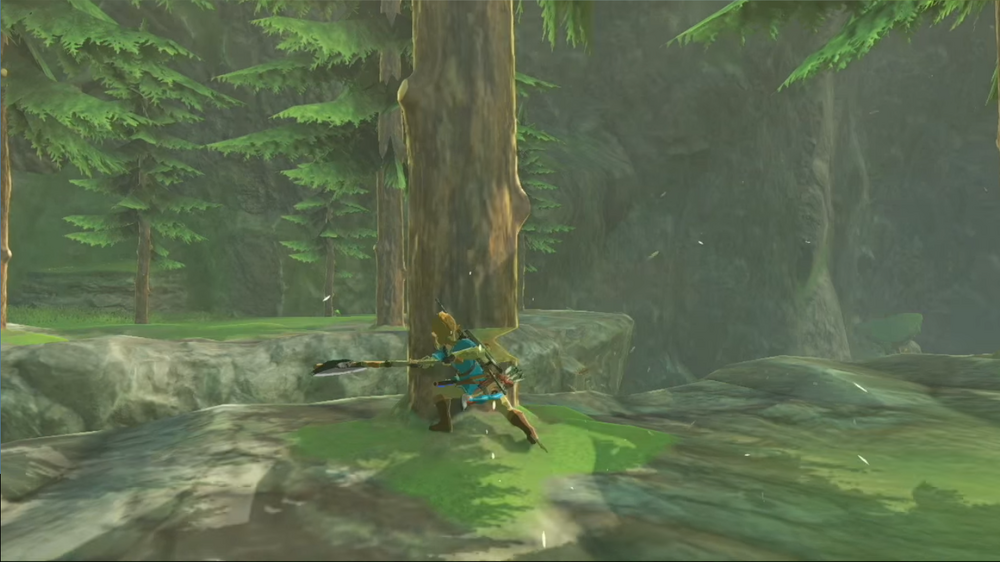
\includegraphics[scale=0.42]{slides/alphabet_trees/link_cut_tree.png}
  \end{center}
}

\frame{
  \frametitle{Link-Cut Tree\footnote{Sleator, D. D.; Tarjan, R. E. (1983).}}
  \begin{columns}
      \begin{column}{0.4\textwidth}
          \begin{itemize}
                  \item Maintains a set of rooted trees

                    \medskip
                  
                    \item Amortized $O(\log n)$ link, cut and find-root at any node

                    \medskip
                    
                    
                    \item Improves Dinic's Algorithm (for max-flow) from $O(V^2E)$ to $O(VE \log V)$.
          \end{itemize}
      \end{column}
        \begin{column}{0.6\textwidth}
            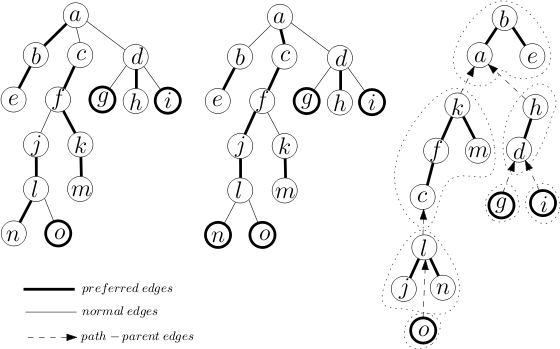
\includegraphics[scale=0.6]{slides/alphabet_trees/Linkcuttree1.png}

            {\tiny By Drrilll, CC BY-SA 3.0, https://commons.wikimedia.org/w/index.php?curid=25495327}
            
        \end{column}
  \end{columns}
    
}